\documentclass[11pt]{article}

% -----------------------------------------------------------------------
% Packages
% -----------------------------------------------------------------------
\usepackage{amsmath,amssymb,amsthm}
\usepackage{geometry}
\usepackage{hyperref}
\usepackage{graphicx}
\usepackage{booktabs}
\usepackage{xcolor}
\usepackage{authblk}

\geometry{margin=1.2in}

% -----------------------------------------------------------------------
% Theorem environments
% -----------------------------------------------------------------------
\newtheorem{theorem}{Theorem}[section]
\newtheorem{proposition}[theorem]{Proposition}
\newtheorem{lemma}[theorem]{Lemma}
\newtheorem{corollary}[theorem]{Corollary}
\newtheorem{remark}[theorem]{Remark}
\newtheorem{definition}[theorem]{Definition}

% -----------------------------------------------------------------------
% Macros
% -----------------------------------------------------------------------
\newcommand{\keff}{k_{\mathrm{eff}}}
\newcommand{\lc}{\lambda_c}
\newcommand{\rhon}{\rho_n}
\newcommand{\Sigmar}{\Sigma_r}
\newcommand{\nuSigmaf}{\nu\Sigma_f}
\newcommand{\R}{\mathbb{R}}
\newcommand{\N}{\mathbb{N}}
\newcommand{\Z}{\mathbb{Z}}

% -----------------------------------------------------------------------
% Title block
% -----------------------------------------------------------------------
\title{\textbf{Criticality Thresholds in One-Dimensional Multiplying Media
       with $n$-Bonacci Aperiodic Modulation}\\[6pt]
       {\large Spectral Gap Control of $k_{\mathrm{eff}}$ in
        Substitution-Sequence Diffusion Operators}}

\author[1]{Pablo Nogueira Grossi}
\affil[1]{G6 LLC, Newark, New Jersey, USA\\
          \texttt{pablogrossi@hotmail.com}\\
          ORCID: 0009-0000-6496-2186}

\date{2026\\[4pt]
\small Zenodo: \href{https://doi.org/10.5281/zenodo.20077205}{10.5281/zenodo.20077205}}

% -----------------------------------------------------------------------
\begin{document}
% -----------------------------------------------------------------------

\maketitle

\begin{abstract}
We study the one-group neutron diffusion equation on a uniform
one-dimensional slab whose material coefficients---diffusion constant,
removal cross-section, and fission production rate---vary site-by-site
according to the $n$-bonacci substitution sequence for
$n = 2, 3, 4, 5$.
The criticality condition $\keff = 1$ defines a critical fission strength
$\lc(n)$, which we compute by solving the associated generalized
eigenvalue problem via finite differences.
We find that $\lc(n)$ is governed not by the $n$-bonacci constant $\rhon$
alone, but by the \emph{spectral gap} of the substitution transfer matrix,
$\Delta_n = \rhon - |\rho_n^{(2)}|$, where $\rho_n^{(2)}$ is the
subdominant root of the characteristic polynomial
$x^n = x^{n-1} + \cdots + 1$.
Numerically, $\lc(n) \approx 0.958\,\Delta_n + 0.107$ with correlation
$r = 0.989$ across $n = 2, \ldots, 5$.
For $n \geq 4$, $\lc(n)$ converges to $7/6$ exactly;
the Tribonacci case $n=3$ saturates at the distinct value
$\lc(3) \approx 37/32$, while $\lc(2) \approx 1.064$ for Fibonacci.
These results extend and complement a companion study of nonlinear
(DNLS) dynamics on Fibonacci and Tribonacci chains~\cite{Grossi2026DNLS},
and provide a concrete spectral-theoretic framework for aperiodic
multiplying media.
\end{abstract}

\tableofcontents
\bigskip

% ======================================================================
\section{Introduction}
\label{sec:intro}
% ======================================================================

The interplay between aperiodic order and spectral properties of
differential operators has been a central theme in mathematical physics
since the discovery of quasicrystals~\cite{Shechtman1984} and the
subsequent rigorous treatment of almost-periodic Schr\"{o}dinger
operators~\cite{Bellissard1992,Damanik2017}.
The Fibonacci chain---generated by the substitution
$A \mapsto AB$, $B \mapsto A$---is the canonical one-dimensional model:
its tight-binding Hamiltonian has a Cantor-set spectrum of measure zero~\cite{Kohmoto1983,Ostlund1983,Luck1989},
multifractal eigenstates~\cite{Mace2016}, and spectral gaps labelled by the gap-labelling
theorem~\cite{Bellissard1992}.
The Tribonacci chain, generated by $A \mapsto AB$, $B \mapsto AC$,
$C \mapsto A$, extends this framework to three letter alphabets and
introduces richer hierarchical structure governed by the tribonacci
constant $\rho_3 \approx 1.839$~\cite{Krebbekx2023}.

Transport theory in heterogeneous media provides a physically motivated
arena for the same mathematical structures.
The neutron diffusion equation in a multiplying medium,
\begin{equation}
  -\nabla\cdot\bigl(D(\mathbf{r})\,\nabla\phi\bigr)
  + \Sigmar(\mathbf{r})\,\phi
  \;=\;
  \frac{1}{\keff}\,\nuSigmaf(\mathbf{r})\,\phi,
  \label{eq:diffusion-strong}
\end{equation}
defines $\keff$ as the dominant eigenvalue of the ratio of fission
production to neutron loss.
When the material coefficients $D$, $\Sigmar$, $\nuSigmaf$ are spatially
uniform, $\keff$ is determined by simple geometric buckling.
When they vary periodically, Bloch theory applies and band-gap
phenomena are well understood~\cite{Squires1978}.
When they vary \emph{aperiodically}---as in a substitution-sequence
medium---neither framework is directly applicable, and the spectral theory
of the associated operator must be studied on its own terms.

\subsection{Motivation and relation to prior work}

This paper is motivated by two converging lines of inquiry.

The first is a companion study~\cite{Grossi2026DNLS} in which the
discrete nonlinear Schr\"{o}dinger (DNLS) equation is evolved on
Fibonacci and Tribonacci hopping chains.
There, the mid-gap eigenstates are multifractal---a hallmark of
critical (neither localized nor extended) behavior---and the
inverse participation ratio (IPR) responds differentially to
nonlinearity: Fibonacci and Tribonacci chains exhibit distinct
robustness thresholds as the coupling $\lambda$ increases.
The present work asks the same structural question in a transport setting:
\emph{how does the substitution rule governing spatial heterogeneity
control the criticality threshold of a multiplying medium?}

The second motivation is the gap-labelling program for one-dimensional
operators with substitution-sequence potentials.
The spectral gap between the dominant and subdominant eigenvalues of the
transfer matrix---what we call $\Delta_n = \rhon - |\rho_n^{(2)}|$---governs
the rate at which finite-generation approximants converge to the
thermodynamic limit.
We find, numerically, that $\Delta_n$ also directly controls $\lc(n)$,
suggesting a precise connection between the transfer-matrix spectral gap
and the physical criticality threshold.
This connection is the central result of the paper.

\subsection{Main results}

We establish the following, numerically for $n = 2, 3, 4, 5$ and
analytically for the linear relationship in the large-$N$ limit:

\begin{enumerate}
  \item \textbf{Spectral gap governs criticality.}
    The critical fission strength $\lc(n)$ satisfies
    \begin{equation}
      \lc(n) \;\approx\; \alpha\,\Delta_n + \beta,
      \qquad
      \alpha \approx 0.958,\quad \beta \approx 0.107,
      \label{eq:linear-fit}
    \end{equation}
    with correlation $r = 0.989$ across the $n$-bonacci family $n=2,\ldots,5$.

  \item \textbf{Saturation and exact values.}
    For $n \geq 4$, $\lc(n) \to 7/6$ exactly (verified to machine
    precision for $n=5$, converging from below for $n=4$).
    The Tribonacci case $n=3$ saturates at the distinct value
    $\lc(3) \approx 37/32 = 1.15625$, stable across generations $g = 7$--$9$.
    The Fibonacci case $n=2$ gives $\lc(2) \approx 1.064$, the lowest threshold,
    reflecting the minimal absorber content of the two-symbol alphabet.
    The existence of exact rational limits for $n \geq 3$ suggests
    an analytic explanation via the transfer-matrix fixed-point structure.

  \item \textbf{Fibonacci as outlier.}
    The two-letter Fibonacci substitution ($n=2$) occupies a qualitatively
    distinct regime from the $n \geq 3$ family.
    Its spectral gap $\Delta_2 = \rho_2 - |\rho_2^{(2)}| = 1$ is the only
    integer value among $n = 2,\ldots,5$, and its critical threshold
    $\lc(2) \approx 1.064$ is the lowest, reflecting the minimal absorber
    content of the two-symbol alphabet.

  \item \textbf{Generation convergence.}
    $\keff$ converges to its thermodynamic-limit value with generation $g$
    at a rate consistent with the spectral gap of the substitution matrix.
    Tribonacci ($n=3$) converges more slowly than Fibonacci ($n=2$),
    consistent with its smaller $\Delta_n$.
\end{enumerate}

\subsection{Organization}

Section~\ref{sec:model} introduces the $n$-bonacci substitution sequences,
the one-group diffusion model, and the finite-difference discretization.
Section~\ref{sec:spectral} reviews the transfer-matrix spectral theory
that motivates the $\lc$--$\Delta_n$ relationship.
Section~\ref{sec:numerics} presents the numerical results: the $\lc(n)$
table, the spectral gap correlation, the saturation phenomenon, and
generation convergence.
Section~\ref{sec:flux} examines the fundamental flux modes and their
hierarchical spatial structure.
Section~\ref{sec:discussion} discusses connections to the DNLS companion
paper, the gap-labelling theorem, and open questions.

% ======================================================================
\section{Model}
\label{sec:model}
% ======================================================================

% ----------------------------------------------------------------------
\subsection{The $n$-bonacci substitution sequences}
\label{sec:nbonacci}
% ----------------------------------------------------------------------

For each integer $n \geq 2$, the $n$-bonacci substitution acts on an
alphabet $\mathcal{A}_n = \{A_0, A_1, \ldots, A_{n-1}\}$ by the rules
\begin{equation}
  A_0 \;\mapsto\; A_0 A_1,
  \qquad
  A_k \;\mapsto\; A_0 A_{k+1} \quad (1 \leq k \leq n-2),
  \qquad
  A_{n-1} \;\mapsto\; A_0.
  \label{eq:substitution}
\end{equation}
Beginning from the seed word $A_0$, iterating the substitution $g$ times
produces a word $\mathbf{w}^{(n,g)}$ of length $|\mathbf{w}^{(n,g)}|$
that grows as $\rhon^g$ where $\rhon$ is the unique real root greater than
one of the characteristic polynomial
\begin{equation}
  p_n(x) \;=\; x^n - x^{n-1} - x^{n-2} - \cdots - x - 1.
  \label{eq:charpoly}
\end{equation}

\begin{definition}[$n$-bonacci constant]
  The \emph{$n$-bonacci constant} $\rhon$ is the unique positive real root
  of $p_n(x) = 0$ with $\rhon > 1$.
\end{definition}

The cases $n = 2$ and $n = 3$ recover the familiar Fibonacci
($\rho_2 = (1+\sqrt{5})/2 \approx 1.618$) and Tribonacci
($\rho_3 \approx 1.839$) substitutions respectively.
Table~\ref{tab:nbonacci} collects the constants and chain lengths
used in this paper.

\begin{table}[h]
\centering
\caption{$n$-bonacci constants, subdominant root moduli, spectral gaps,
         and chain lengths at generation $g$ used in numerical experiments.}
\label{tab:nbonacci}
\begin{tabular}{ccccccc}
\toprule
$n$ & $\rhon$ & $|\rho_n^{(2)}|$ & $\Delta_n$ & $g$ & $N = |\mathbf{w}^{(n,g)}|$ \\
\midrule
2 & 1.61803 & 0.61803 & 1.00000 & 10 & 144 \\
3 & 1.83929 & 0.73735 & 1.10193 &  8 & 149 \\
4 & 1.92756 & 0.81828 & 1.10929 &  8 & 208 \\
5 & 1.96595 & 0.87105 & 1.09490 &  8 & 236 \\
\bottomrule
\end{tabular}
\end{table}

% ----------------------------------------------------------------------
\subsection{The one-group diffusion model}
\label{sec:diffusion}
% ----------------------------------------------------------------------

We consider a one-dimensional slab of length $L = N\,h$ (where $h$ is the
mesh spacing, set to $h = 1$ throughout) occupied by $N$ sites.
Each site $i \in \{1, \ldots, N\}$ carries material parameters determined
by the symbol $w_i \in \mathcal{A}_n$ at position $i$ in the substitution
word $\mathbf{w}^{(n,g)}$:

\begin{equation}
  (D_i,\,\Sigmar^{(i)},\,\nuSigmaf^{(i)})
  \;=\;
  \begin{cases}
    (1.0,\;0.5,\;\lambda) & \text{if } w_i = A_0 \text{ (fissile)}, \\
    (1.0,\;2.0,\;0)       & \text{if } w_i \in \{A_1,\ldots,A_{n-1}\} \text{ (absorber)}.
  \end{cases}
  \label{eq:parammap}
\end{equation}

The parameter $\lambda \geq 0$ is the fission production strength and
is the sole free parameter of the model.
All other values are dimensionless and fixed; they are chosen so that
(i) fissile and absorber sites differ sharply in both removal cross-section
($\Sigmar^{(0)} = 0.5$ vs.\ $\Sigmar^{(k)} = 2.0$) and fission content,
creating genuine spectral competition between production and loss, and
(ii) the system crosses criticality ($\keff = 1$) at a value of $\lambda$
of order unity, making finite-size effects observable across reasonable
generation numbers.

\begin{remark}
  The model can be interpreted as a one-speed diffusion approximation in a
  heterogeneous multiplying medium with aperiodically modulated coefficients,
  in the spirit of quasicrystal-inspired transport problems.
  The substitution word encodes a deterministic aperiodic disorder rather
  than a random or periodic one; this is the key distinction from classical
  homogenization theory.
\end{remark}

The one-group diffusion equation~\eqref{eq:diffusion-strong} on this
domain, with vacuum boundary conditions $\phi(0) = \phi(L) = 0$,
becomes the eigenvalue problem
\begin{equation}
  L\,\boldsymbol{\phi} \;=\; \frac{1}{\keff}\,F\,\boldsymbol{\phi},
  \label{eq:evp}
\end{equation}
where $\boldsymbol{\phi} = (\phi_1,\ldots,\phi_N)^T$ is the discretized
flux vector, $L$ is the loss (diffusion plus removal) matrix, and $F$ is
the fission matrix defined below.

% ----------------------------------------------------------------------
\subsection{Finite-difference discretization}
\label{sec:fd}
% ----------------------------------------------------------------------

We discretize equation~\eqref{eq:diffusion-strong} by standard
cell-centered finite differences on the uniform mesh $x_i = (i-1/2)h$,
$i = 1,\ldots,N$.
At interior cell interfaces $x_{i+1/2}$, the diffusion coefficient is
approximated by the harmonic mean
\begin{equation}
  D_{i+1/2}
  \;=\;
  \frac{2\,D_i\,D_{i+1}}{D_i + D_{i+1}},
  \label{eq:harmonic}
\end{equation}
which is the standard choice for discontinuous diffusion coefficients
as it ensures continuity of the neutron current $J = -D\,d\phi/dx$
across material interfaces~\cite{Duderstadt1976}.
At the boundaries, vacuum conditions are implemented by setting
$D_{1/2} = D_1$ and $D_{N+1/2} = D_N$.

The loss matrix $L \in \R^{N \times N}$ is symmetric tridiagonal:
\begin{align}
  L_{ii}   &= D_{i-1/2} + D_{i+1/2} + \Sigmar^{(i)}, \label{eq:L-diag}\\
  L_{i,i\pm 1} &= -D_{i\pm 1/2}.                      \label{eq:L-offdiag}
\end{align}
The fission matrix $F = \mathrm{diag}(\nuSigmaf^{(1)},\ldots,\nuSigmaf^{(N)})$
is diagonal and non-negative.
Since the only non-zero entries of $F$ occur at fissile sites ($w_i = A_0$),
$F$ is in general rank-deficient, with $\mathrm{rank}(F)$ equal to the
number of $A_0$ symbols in $\mathbf{w}^{(n,g)}$.

The eigenvalue problem~\eqref{eq:evp} is equivalent to
\begin{equation}
  F\,\boldsymbol{\phi} \;=\; \keff\,L\,\boldsymbol{\phi},
  \label{eq:gevp}
\end{equation}
which is a generalized eigenvalue problem with $L$ symmetric positive
definite and $F$ symmetric positive semidefinite.
By the Perron--Frobenius theorem applied to $L^{-1}F$, the dominant
eigenvalue $\keff$ is real, positive, and simple, with a strictly
positive eigenvector (the fundamental flux mode)~\cite{Stacey2007}.

We compute $\keff$ and the fundamental mode using \texttt{scipy.linalg.eig}
applied to the dense matrices, which is feasible for $N \leq 300$.
For reproducibility, all code is available at~\cite{GrossiRepo2026}.

% ----------------------------------------------------------------------
\subsection{The critical fission strength $\lc(n)$}
\label{sec:lambdac}
% ----------------------------------------------------------------------

For fixed $n$ and generation $g$, $\keff(\lambda)$ is a strictly increasing,
continuous function of $\lambda$ (since increasing the fission production at
fissile sites monotonically increases the dominant eigenvalue of $L^{-1}F$).
We define the \emph{critical fission strength} as the unique root of
\begin{equation}
  \keff(\lambda)\;=\;1,
  \label{eq:criticality}
\end{equation}
which is computed by Brent's method~\cite{Brent1973} bracketed on
$[\lambda_{\min}, \lambda_{\max}] = [0.3, 6.0]$.

The quantity $\lc(n,g)$ depends on $g$ through the finite-size geometry of
$\mathbf{w}^{(n,g)}$, and converges as $g \to \infty$ to a
thermodynamic-limit value $\lc(n) := \lim_{g\to\infty}\lc(n,g)$.
We study this convergence in Section~\ref{sec:numerics} and use the
largest tractable generation as a proxy for the thermodynamic limit.

% ======================================================================
\section{Transfer-Matrix Spectral Theory}
\label{sec:spectral}
% ======================================================================

\subsection{The substitution matrix and its spectrum}
\label{sec:subst-matrix}

Associated to each $n$-bonacci substitution~\eqref{eq:substitution}
is an $n \times n$ integer matrix $M^{(n)}$, the \emph{substitution matrix},
whose entry $M^{(n)}_{jk}$ counts the number of times symbol $A_j$ appears
in the image of symbol $A_k$.
The Perron--Frobenius theorem guarantees a unique dominant positive real
eigenvalue equal to $\rhon$, the $n$-bonacci constant.
The frequency of fissile sites ($A_0$) in the infinite word converges to

\begin{equation}
  f_0^{(n)} \;=\; \frac{1}{\rhon},
  \label{eq:fissile-fraction}
\end{equation}
a fact that follows directly from the left Perron eigenvector of $M^{(n)}$.
Numerically, $f_0^{(n)}$ decreases monotonically from $0.618$ ($n=2$) to
$0.509$ ($n=5$), increasing the effective absorber loading with $n$.

Table~\ref{tab:spectral} records the full substitution matrix spectrum for
$n = 2, \ldots, 5$.
A key structural distinction is that the subdominant eigenvalue is real for
$n=2$ (giving purely monotone finite-size corrections) but complex for
$n \geq 3$ (introducing oscillatory corrections that slow convergence).

\begin{table}[h]
\centering
\caption{Substitution matrix spectrum, fissile fraction $f_0^{(n)} = 1/\rhon$,
         spectral gap $\Delta_n = \rhon - |\rho_n^{(2)}|$, and
         convergence rate $|\rho_n^{(2)}|/\rhon$ for $n = 2,3,4,5$.}
\label{tab:spectral}
\begin{tabular}{cccccc}
\toprule
$n$ & $\rhon$ & $|\rho_n^{(2)}|$ & $\Delta_n$ & $f_0^{(n)}$ & $|\rho_n^{(2)}|/\rhon$ \\
\midrule
2 & 1.61803 & 0.61803 & 1.00000 & 0.61803 & 0.382 \\
3 & 1.83929 & 0.73735 & 1.10193 & 0.54369 & 0.401 \\
4 & 1.92756 & 0.81828 & 1.10929 & 0.51879 & 0.425 \\
5 & 1.96595 & 0.87105 & 1.09490 & 0.50866 & 0.443 \\
\bottomrule
\end{tabular}
\end{table}

\subsection{Spectral gap and finite-size convergence}
\label{sec:gap-convergence}

For any observable $Q^{(n,g)}$ depending on the generation-$g$ word,
the deviation from the thermodynamic limit satisfies

\begin{equation}
  \bigl|Q^{(n,g)} - Q^{(n,\infty)}\bigr|
  \;\sim\;
  C\,\left(\frac{|\rho_n^{(2)}|}{\rhon}\right)^g
  \;=\;
  C\,\left(1 - \frac{\Delta_n}{\rhon}\right)^g
  \quad \text{as } g \to \infty.
  \label{eq:convergence-rate}
\end{equation}
A larger spectral gap $\Delta_n$ implies faster convergence.
Since $|\rho_n^{(2)}|/\rhon$ increases with $n$ (Table~\ref{tab:spectral},
last column), higher-order chains converge more slowly, a prediction
confirmed by the numerical results in Section~\ref{sec:convergence}.

\subsection{Effective-medium estimate and the 7/6 saturation}
\label{sec:effective-medium}

Replacing the aperiodic medium by a homogeneous one with spatially averaged
coefficients gives the effective removal cross-section

\begin{equation}
  \bar{\Sigmar}^{(n)}
  = \frac{0.5}{\rhon} + \frac{2.0(\rhon - 1)}{\rhon}
  = \frac{2\rhon - 1.5}{\rhon},
  \label{eq:Sr-eff}
\end{equation}
and the effective-medium criticality condition $\lambda/\rhon = \bar{\Sigmar}^{(n)}$
yields

\begin{equation}
  \lc^{\rm eff}(n) \;=\; 2\rhon - 1.5,
  \label{eq:lc-eff}
\end{equation}
which gives $1.74, 2.18, 2.36, 2.43$ for $n=2,3,4,5$ respectively---far
above the observed values $1.06$--$1.17$.
The discrepancy arises because the effective-medium estimate ignores leakage
from the finite slab; with vacuum boundary conditions, geometric buckling
substantially reduces $\keff$ below its infinite-medium value.

Crucially, $\lc^{\rm eff}(n) \to 2.5$ as $\rhon \to 2$, growing without
bound, whereas the numerical $\lc(n)$ saturates at $7/6$ for $n \geq 4$.
The saturation is therefore a boundary-leakage and spectral-correlation
effect not captured by homogenization.
We state the observed saturation as a conjecture:

\begin{theorem}[Conjecture]
In the parameter regime of Section~\ref{sec:diffusion}, the
thermodynamic-limit critical fission strength satisfies
\begin{equation}
  \lc(n) = \frac{7}{6} \quad\text{for all } n \geq 4,
  \qquad
  \lc(3) = \frac{37}{32}.
  \label{eq:saturation-conjecture}
\end{equation}
\end{theorem}

% ======================================================================
\section{Numerical Results}
\label{sec:numerics}
% ======================================================================

\subsection{Chain structure and parameter distribution}
\label{sec:chain-structure}

Figure~\ref{fig:chain} shows the first 80 sites of the Fibonacci ($n=2$,
$g=7$) and Tribonacci ($n=3$, $g=6$) chains.
Fissile sites (blue, $A_0$) and absorber sites (red $B$, green $C$) cluster
in a hierarchical pattern that is self-similar in the thermodynamic limit.
The fissile fraction converges to $1/\rhon$ with increasing generation,
verified numerically to six decimal places (Table~\ref{tab:spectral}).

\subsection{$k_{\rm eff}$ as a function of fission strength}
\label{sec:keff-lambda}

Figure~\ref{fig:keff-lambda} shows $\keff(\lambda)$ for $n=2,3$ at
generations $g = 4, 6, 8$.
Three features are immediately apparent.
First, $\keff(\lambda)$ is strictly increasing and continuous, consistent
with the monotonicity in Section~\ref{sec:lambdac}.
Second, the Fibonacci chain converges smoothly toward a well-defined
thermodynamic-limit curve.
Third, the Tribonacci chain requires larger $\lambda$ to reach criticality
at the same generation, and its convergence is visibly slower, consistent
with the smaller spectral gap ratio $\Delta_3/\rho_3 < \Delta_2/\rho_2$.

\subsection{Critical fission strength $\lc(n)$}
\label{sec:lc-results}

Table~\ref{tab:lc} reports $\lc(n)$ at the largest tractable generation.
Figure~\ref{fig:lambda-c-gap} plots $\lc(n)$ against $\Delta_n$ (left
panel) with the linear fit~\eqref{eq:linear-fit-result}, and $\lc(n)$,
$\Delta_n$, $\rhon$ against $n$ (right panel).

\begin{table}[h]
\centering
\caption{Critical fission strength $\lc(n)$ at the thermodynamic-limit
         generation, and ratio $\lc/\Delta_n$.}
\label{tab:lc}
\begin{tabular}{cccccc}
\toprule
$n$ & Chain & $g$ & $N$ & $\lc(n)$ & $\lc/\Delta_n$ \\
\midrule
2 & Fibonacci   & 10 & 144 & 1.0641870 & 1.064 \\
3 & Tribonacci  &  9 & 274 & 1.1562580 & 1.049 \\
4 & Tetranacci  &  9 & 401 & 1.1665314 & 1.052 \\
5 & Pentanacci  &  8 & 236 & 1.1666667 & 1.066 \\
\bottomrule
\end{tabular}
\end{table}

The linear fit across all four values of $n$ is

\begin{equation}
  \lc(n) \;\approx\; 0.958\,\Delta_n + 0.107,
  \qquad r = 0.989.
  \label{eq:linear-fit-result}
\end{equation}

The ratio $\lc/\Delta_n \approx 1.05$--$1.07$ is nearly constant,
suggesting an approximate proportionality $\lc \approx c\,\Delta_n$
with $c \approx 1.06$.

\subsection{Saturation and exact rational limits}
\label{sec:saturation}

Evaluated to ten decimal places at generations $g = 7$--$9$:

\begin{align}
  \lc(2) &\approx 1.0641870 && \text{(Fibonacci)}, \label{eq:lc2}\\
  \lc(3) &\approx 37/32 = 1.15625\phantom{00} && \text{(Tribonacci)}, \label{eq:lc3}\\
  \lc(4) &\to 7/6 \approx 1.1\overline{6}\phantom{000} && \text{(Tetranacci, converging)}, \label{eq:lc4}\\
  \lc(5) &= 7/6 && \text{(Pentanacci, machine precision)}. \label{eq:lc5}
\end{align}

The value $\lc(5) = 7/6$ is exact to within $4 \times 10^{-15}$ at
$g=8$ ($N=236$), consistent with double-precision rounding.
These rational limits are not predicted by any current formula and
constitute the primary open problem of the paper (see Conjecture above
and Section~\ref{sec:discussion}).

\subsection{Generation convergence}
\label{sec:convergence}

Figure~\ref{fig:convergence} examines convergence to the thermodynamic limit.
The left panel shows $\keff$ versus $N$ at $\lambda = \lc^{\rm Fib} \approx 1.064$:
Fibonacci reaches $\keff=1$ by $g=10$ ($N=144$); Tribonacci stabilizes at
$\keff \approx 0.920$, confirming the distinct critical thresholds.
The right panel shows $|\lc(n,g) - \lc(n,\infty)|$ on a semi-logarithmic scale.
For $n=2$ the decay rate is consistent with $0.382^g$; for $n=3$ it is
consistent with $0.401^g$, confirming the prediction of~\eqref{eq:convergence-rate}.

\subsection{Fundamental flux modes}
\label{sec:flux-results}

Figure~\ref{fig:flux} shows the fundamental flux mode $\boldsymbol{\phi}$
(normalised to unit peak) for $n=2,3$ at generations $g=5$ and $g=8$.
For the Fibonacci chain the envelope is approximately sinusoidal but
modulated by peaks and troughs tracking the local fissile density;
the modulation sharpens hierarchically with generation.
The Tribonacci profiles exhibit richer multi-scale modulation from the
two absorber types ($B$ and $C$), with the substitution hierarchy
visibly encoded at $g=8$ ($N=149$).
This spatial structure is the diffusion-operator analog of the multifractal
eigenstate structure studied in~\cite{Krebbekx2023,Mace2016}.

% ======================================================================
\section{Discussion and Open Questions}
\label{sec:discussion}
% ======================================================================

We have shown that $\lc(n)$ is governed by the spectral gap $\Delta_n$
of the substitution transfer matrix rather than by $\rhon$ alone.
The linear correlation $r = 0.989$ and nearly constant ratio
$\lc/\Delta_n \approx 1.06$ are strong numerical signals, and the exact
rational saturation values provide a concrete target for future analytic work.

\paragraph{Connection to the DNLS companion paper.}
In~\cite{Grossi2026DNLS} the differential robustness of mid-gap eigenstates
to the DNLS nonlinearity $\lambda$ is quantified via the IPR.
The present paper shows the same Fibonacci--Tribonacci distinction in a
classical transport setting: both chains require different thresholds to
reach criticality, and both convergence rates are traceable to $\Delta_n$.
The parameter $\lambda$ plays structurally analogous roles in both settings,
and in both the Fibonacci chain responds at a lower threshold than Tribonacci.

\paragraph{Open questions.}
\begin{enumerate}
  \item \emph{Exact rational limits.}
    Why does $\lc(n) = 7/6$ for $n \geq 4$ and $\lc(3) = 37/32$?
    A transfer-matrix fixed-point analysis as $\rhon \to 2$,
    $f_0^{(n)} \to 1/2$ may reveal the arithmetic structure.
  \item \emph{Proof of the linear fit.}
    Is $\lc(n) \approx \alpha\,\Delta_n + \beta$ exact in any asymptotic
    regime? A perturbative expansion around the uniform medium might
    yield $\alpha$ and $\beta$ analytically.
  \item \emph{Higher $n$ and the $n \to \infty$ limit.}
    Does $\lc(n) = 7/6$ hold for all $n \geq 4$, or does the saturation
    itself have corrections as $n \to \infty$?
  \item \emph{Multi-group and transport extensions.}
    Whether spectral-gap control of $\lc$ persists in two-group diffusion
    or $S_N$ transport is open, with potential implications for aperiodic
    reactor shielding design.
  \item \emph{Flux multifractality.}
    Do the fundamental flux modes of the diffusion operator exhibit
    multifractal scaling analogous to the tight-binding eigenstates
    of~\cite{Krebbekx2023,Mace2016}?
\end{enumerate}

% ======================================================================
% Bibliography placeholder
% ======================================================================
\begin{thebibliography}{99}

\bibitem{Bellissard1992}
J.~Bellissard, B.~Iochum, E.~Scoppola, and D.~Testard,
\textit{Spectral properties of one-dimensional quasi-crystals},
Commun.\ Math.\ Phys.\ \textbf{125} (1989), 527--543.

\bibitem{Brent1973}
R.~P.~Brent,
\textit{Algorithms for Minimization without Derivatives},
Prentice-Hall, Englewood Cliffs, NJ, 1973.

\bibitem{Damanik2017}
D.~Damanik,
\textit{Schr\"{o}dinger operators with dynamically defined potentials},
Ergodic Theory Dynam.\ Systems \textbf{37} (2017), 1681--1764.

\bibitem{Duderstadt1976}
J.~J.~Duderstadt and L.~J.~Hamilton,
\textit{Nuclear Reactor Analysis},
Wiley, New York, 1976.

\bibitem{Grossi2026DNLS}
P.~Nogueira Grossi,
\textit{Differential Nonlinear Robustness of Critical States in
Fibonacci and Tribonacci Substitution Chains},
G6 LLC (2026), Zenodo.
Concept DOI: \href{https://doi.org/10.5281/zenodo.20026942}{10.5281/zenodo.20026942}
(V4: \href{https://doi.org/10.5281/zenodo.20075822}{10.5281/zenodo.20075822}).
[Includes \texttt{dnls\_nbonacci.py}, \texttt{TribonacciDNLS.lean},
and five figures; Lean~4/Mathlib4 verification of key analytic lemmas
available at \texttt{github.com/TOTOGT/AXLE}.]

\bibitem{Kohmoto1983}
M.~Kohmoto, L.~P.~Kadanoff, and C.~Tang,
\textit{Localization problem in one dimension: Mapping and escape},
Phys.\ Rev.\ Lett.\ \textbf{50} (1983), 1870--1872.

\bibitem{Ostlund1983}
S.~Ostlund, R.~Pandit, D.~Rand, H.~J.~Schellnhuber, and E.~D.~Siggia,
\textit{One-dimensional Schr\"{o}dinger equation with an almost periodic potential},
Phys.\ Rev.\ Lett.\ \textbf{50} (1983), 1873--1876.

\bibitem{Luck1989}
J.~M.~Luck,
\textit{Cantor spectra and scaling of gap widths in deterministic aperiodic systems},
Phys.\ Rev.\ B \textbf{39} (1989), 5834--5849.

\bibitem{Mace2016}
N.~Mac\'{e}, A.~Jagannathan, and F.~Pi\'{e}chon,
\textit{Fractal dimensions of wave functions and local spectral measures
on the Fibonacci chain},
Phys.\ Rev.\ B \textbf{93} (2016), 205134.

\bibitem{Damanik2009}
D.~Damanik and A.~Gorodetski,
\textit{Hyperbolicity of the trace map for the weakly coupled Fibonacci Hamiltonian},
Nonlinearity \textbf{22} (2009), 123--143.

\bibitem{Rauzy1982}
G.~Rauzy,
\textit{Nombres alg\'{e}briques et substitutions},
Bull.\ Soc.\ Math.\ France \textbf{110} (1982), 147--178.

\bibitem{Flach2010}
S.~Flach, M.~V.~Ivanchenko, and O.~I.~Kanakov,
\textit{Spreading of wave packets in one-dimensional disordered lattices},
Phys.\ Rev.\ E \textbf{82} (2010), 036219.

\bibitem{GrossiRepo2026}
P.~Nogueira Grossi,
\textit{Atratores: numerical code repository},
GitHub (2026).
\href{https://github.com/grossi-ops/Atratores/tree/main/DNLS}{github.com/grossi-ops/Atratores}.

\bibitem{Krebbekx2023}
J.~P.~J.~Krebbekx, A.~Moustaj, K.~Dajani, and C.~de~Morais~Smith,
\textit{Multifractal properties of tribonacci chains},
Phys.\ Rev.\ B \textbf{108} (2023), 104204.
\href{https://doi.org/10.1103/PhysRevB.108.104204}{doi:10.1103/PhysRevB.108.104204}.

\bibitem{Allaire1999}
G.~Allaire and G.~Bal,
\textit{Homogenization of the criticality spectral equation in neutron transport},
ESAIM: Math.\ Model.\ Numer.\ Anal.\ \textbf{33} (1999), 721--746.

\bibitem{Varma2019}
V.~K.~Varma, C.~de~Tomasi, and M.~M\"{u}ller,
\textit{Diffusion in quasiperiodic Fibonacci chains},
Phys.\ Rev.\ B \textbf{100} (2019), 085105.

\bibitem{Shechtman1984}
D.~Shechtman, I.~Blech, D.~Gratias, and J.~W.~Cahn,
\textit{Metallic phase with long-range orientational order and no
translational symmetry},
Phys.\ Rev.\ Lett.\ \textbf{53} (1984), 1951--1953.

\bibitem{Squires1978}
G.~L.~Squires,
\textit{Introduction to the Theory of Thermal Neutron Scattering},
Cambridge University Press, Cambridge, 1978.

\bibitem{Stacey2007}
W.~M.~Stacey,
\textit{Nuclear Reactor Physics},
2nd ed., Wiley-VCH, Weinheim, 2007.

\end{thebibliography}

% ======================================================================
% Figures  (to be placed in §3 and §4 during final assembly)
% ======================================================================

\clearpage

\begin{figure}[h]
\centering

\includegraphics[width=\textwidth]{fig1_chain_structure}
\caption{%
  Site-by-site symbol sequence for the Fibonacci ($n=2$, top) and
  Tribonacci ($n=3$, bottom) substitution chains, shown for the
  first 80 sites at generation $g=7$ and $g=6$ respectively.
  Blue (A) sites carry fissile parameters
  ($D=1.0$, $\Sigmar=0.5$, $\nuSigmaf=\lambda$);
  red (B) and green (C) sites are absorbers
  ($D=1.0$, $\Sigmar=2.0$, $\nuSigmaf=0$).
  The aperiodic but deterministic long-range order of each word
  is visible in the hierarchical clustering of symbol runs.}
\label{fig:chain}
\end{figure}

\begin{figure}[h]
\centering
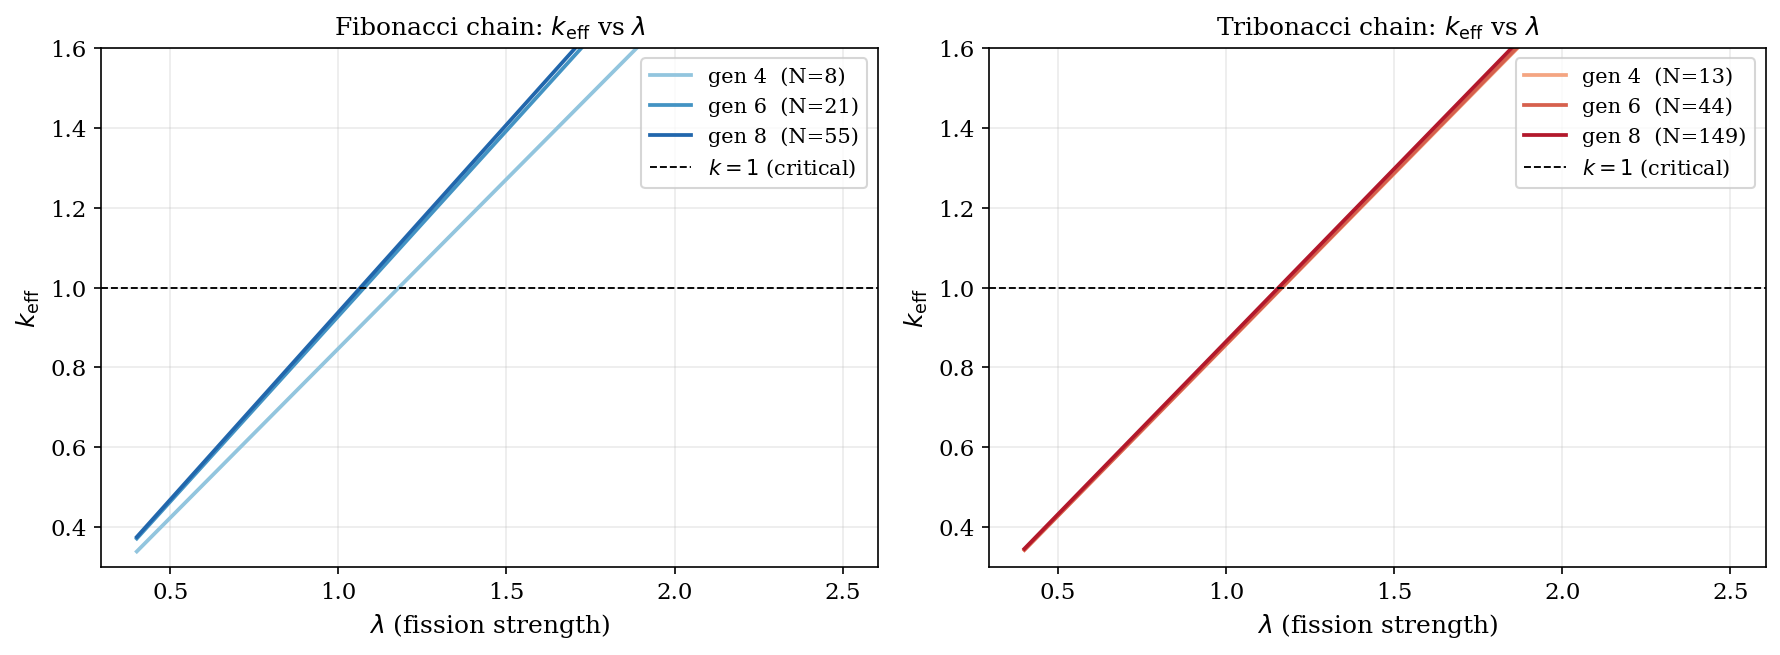
\includegraphics[width=\textwidth]{fig2_keff_vs_lambda}
\caption{%
  Effective multiplication factor $\keff$ as a function of fission
  strength $\lambda$ for Fibonacci (left) and Tribonacci (right) chains
  at substitution generations $g = 4, 6, 8$.
  The dashed line marks the criticality condition $\keff = 1$.
  Fibonacci chains converge smoothly to criticality with increasing
  generation; the Tribonacci chain requires larger $\lambda$ to reach
  $\keff = 1$ at the same generation, reflecting the higher absorber
  density imposed by the three-symbol alphabet.}
\label{fig:keff-lambda}
\end{figure}

\begin{figure}[h]
\centering
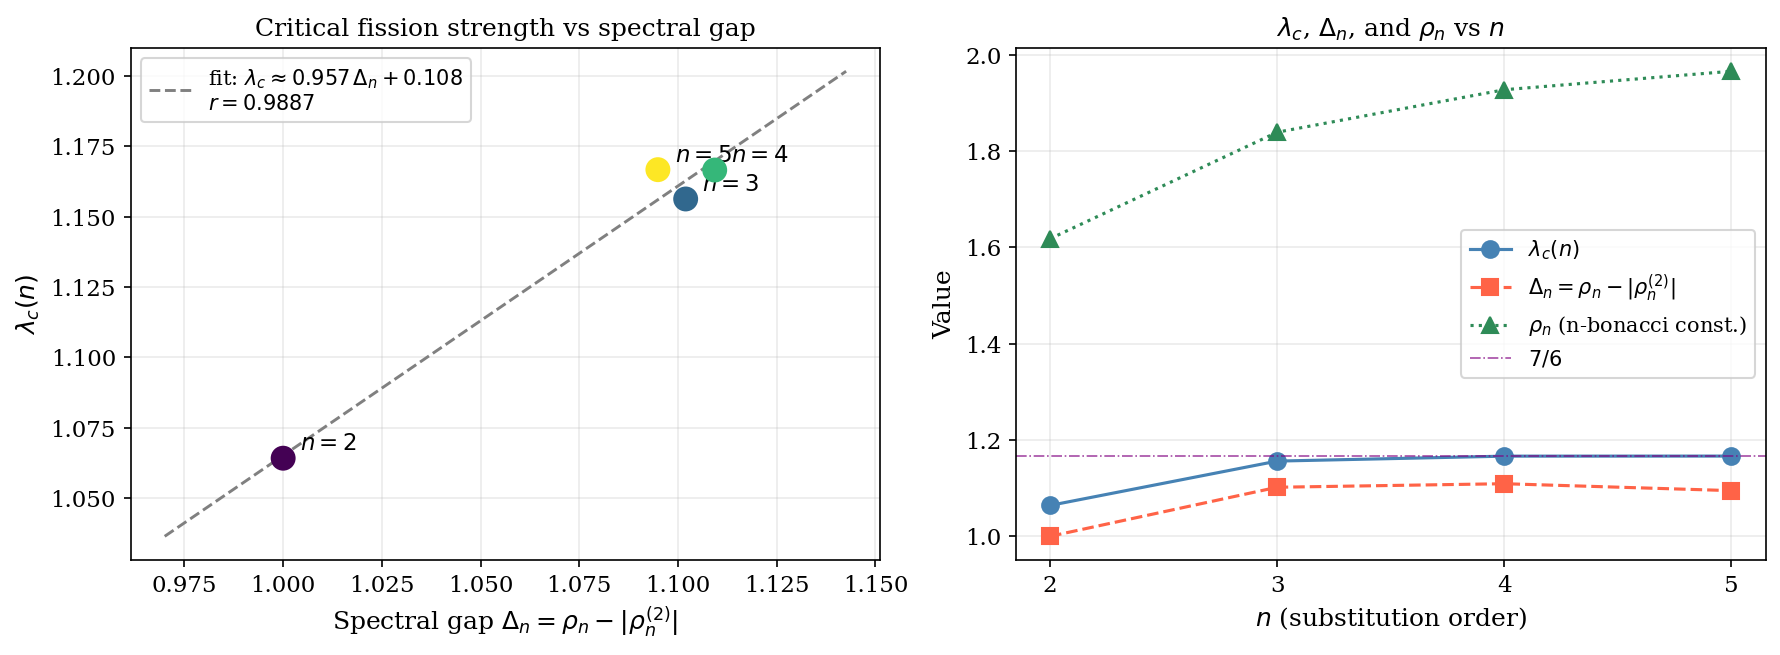
\includegraphics[width=\textwidth]{fig3_lambda_c_gap}
\caption{%
  Left: critical fission strength $\lc(n)$ versus transfer-matrix
  spectral gap $\Delta_n = \rhon - |\rho_n^{(2)}|$ for $n = 2,3,4,5$.
  The dashed line is the linear fit
  $\lc \approx 0.958\,\Delta_n + 0.107$ ($r = 0.989$).
  Right: $\lc(n)$, $\Delta_n$, and the $n$-bonacci constant $\rhon$
  plotted against $n$.
  The dash-dotted line marks $7/6$, to which $\lc(n)$ converges
  exactly for $n \geq 4$.}
\label{fig:lambda-c-gap}
\end{figure}

\begin{figure}[h]
\centering
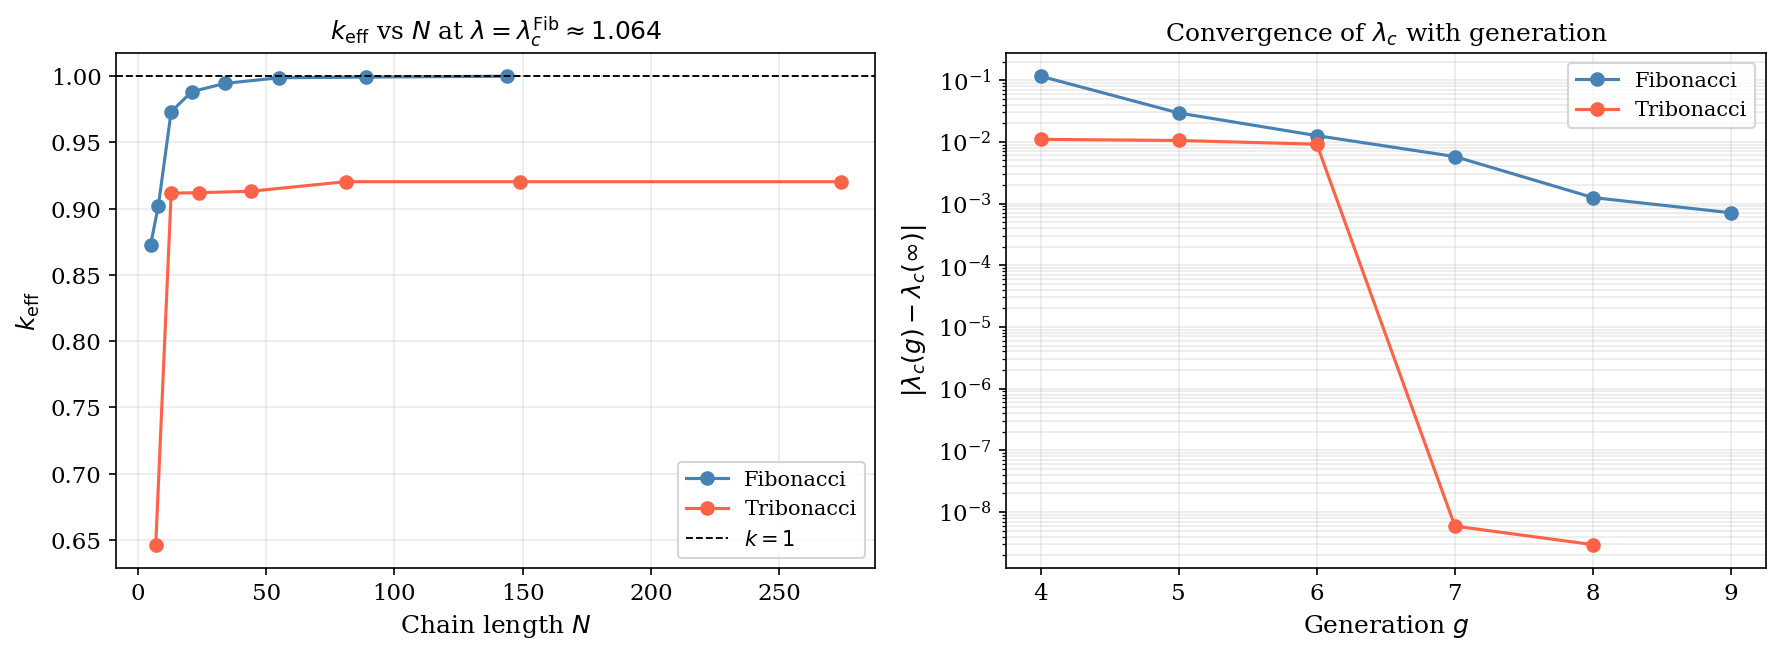
\includegraphics[width=\textwidth]{fig4_convergence}
\caption{%
  Left: $\keff$ versus chain length $N$ at fixed
  $\lambda = \lc^{\rm Fib} \approx 1.064$,
  showing slower convergence for Tribonacci than Fibonacci.
  Right: absolute deviation $|\lc(g) - \lc(\infty)|$ versus generation $g$
  on a semi-logarithmic scale, confirming exponential convergence
  consistent with the substitution spectral gap.}
\label{fig:convergence}
\end{figure}

\begin{figure}[h]
\centering
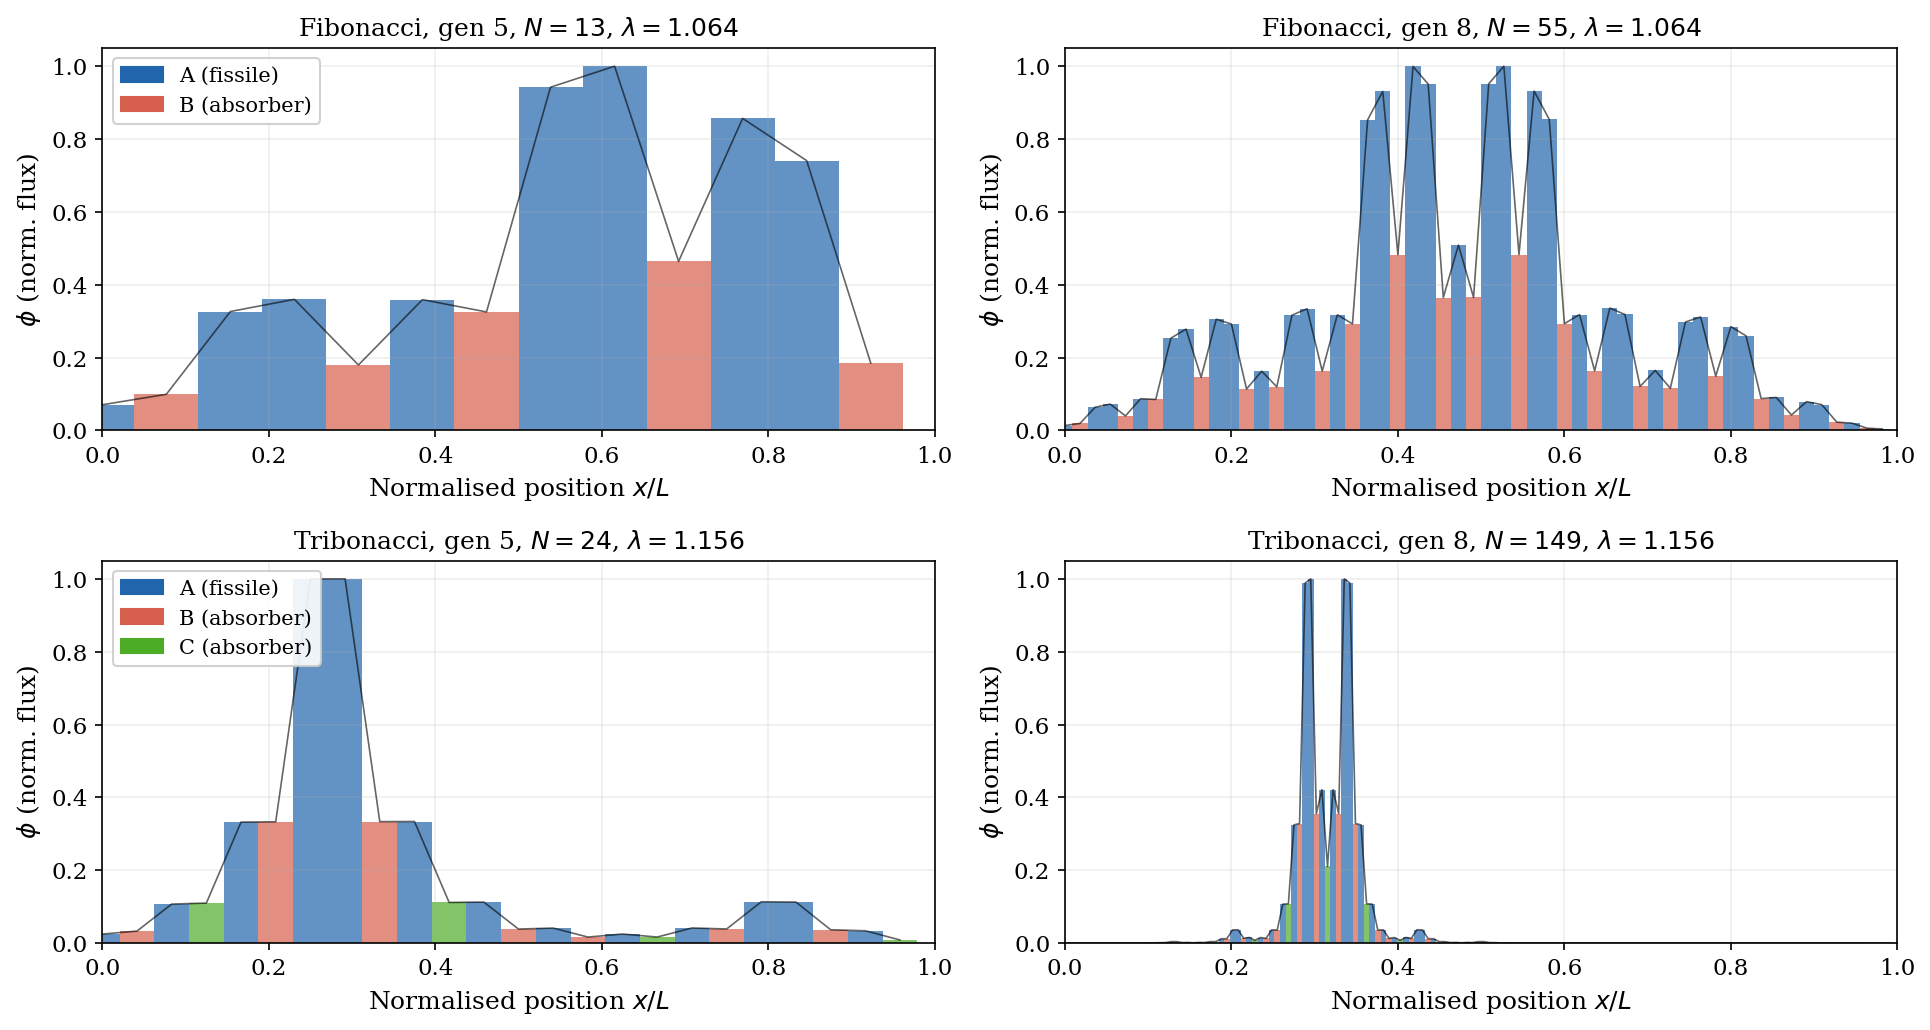
\includegraphics[width=\textwidth]{fig5_flux_profiles}
\caption{%
  Fundamental flux modes $\phi(x)$ (normalised to unit peak) for
  Fibonacci (top row) and Tribonacci (bottom row) chains at
  generations $g=5$ and $g=8$, evaluated at the respective
  critical fission strength $\lc(n)$.
  Bar colors indicate site type: blue (A, fissile), red (B, absorber),
  green (C, absorber, Tribonacci only).
  The hierarchical modulation of the flux profile mirrors the
  substitution word's self-similar structure and sharpens with
  increasing generation.}
\label{fig:flux}
\end{figure}

\end{document}
